% Nallino, Part I p. 188: Ptolemy's figure for the ascensional difference (Almagest II, 7), redrawn from the print:
% the meridian ABGD as a circle; the horizon BED and the equator AEG as flat arcs of circles, as printed; the arcs
% ZHT and LKZ of the circles of declination through the south pole Z; the axis through E in dashes, each where it
% printed; the upright bold letters and the italic words horizon and aequator. Measured on the scan
% (_intake/latin/tools/fig188).
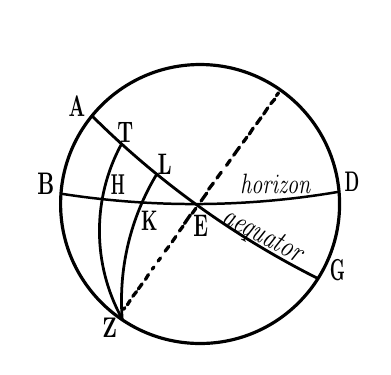
\begin{tikzpicture}[x=0.9928pt,y=-0.9928pt,line cap=butt,every node/.style={font=\fontsize{11}{11}\bfseries\itshape\selectfont,inner sep=0pt}]
\useasboundingbox (0,0) rectangle (122.00,116.00);
\draw[line width=1.15pt] (62.75,64.18) circle[radius=50.77];  % the meridian ABGD
\draw[line width=0.90pt] (12.11,60.42) arc[start angle=98.92,end angle=80.29,radius=312.69];
\draw[line width=1.02pt] (23.40,32.09) arc[start angle=134.85,end angle=116.65,radius=320.45];
\draw[line width=1.00pt] (34.39,106.00) arc[start angle=151.05,end angle=208.53,radius=66.22];
\draw[line width=1.00pt] (46.97,53.34) arc[start angle=-148.87,end angle=-184.26,radius=89.05];
% the dashes of the axis
\draw[line width=1.19pt,line cap=round] (89.97,25.97)--(88.50,27.65) (87.38,29.18)--(85.91,31.45) (84.92,32.77)--(83.31,35.00) (82.07,36.54)--(80.68,38.74) (79.79,39.85)--(78.45,41.69) (77.08,43.48)--(74.99,46.43) (73.73,48.17)--(72.38,50.12) (70.44,52.62)--(68.91,54.73);
\draw[line width=1.19pt,line cap=round] (67.59,56.55)--(65.86,58.81) (59.21,68.12)--(57.09,71.28) (56.55,72.27)--(55.24,74.01) (53.93,76.01)--(52.58,77.96) (51.37,79.63)--(50.02,81.34) (48.35,83.83)--(47.48,84.93) (45.95,87.13)--(45.33,87.89) (43.94,89.87)--(42.88,91.65);
\draw[line width=1.19pt,line cap=round] (41.63,93.25)--(40.29,95.09) (39.61,96.07)--(38.26,97.78) (37.28,99.26)--(36.28,100.88) (91.30,23.70)--(90.56,24.73) (65.18,60.21)--(63.10,63.12) (61.22,65.74)--(59.90,67.60) (35.35,101.91)--(34.90,102.54);
\node at (17.92,28.51) {\normalfont\fontsize{11}{11}\bfseries\selectfont \resizebox{5.99pt}{7.38pt}{A}};
\node at (35.50,38.21) {\normalfont\fontsize{11}{11}\bfseries\selectfont \resizebox{5.74pt}{7.36pt}{T}};
\node at (49.84,49.61) {\normalfont\fontsize{11}{11}\bfseries\selectfont \resizebox{5.10pt}{7.36pt}{L}};
\node at (6.64,56.89) {\normalfont\fontsize{11}{11}\bfseries\selectfont \resizebox{6.12pt}{7.74pt}{B}};
\node at (32.82,57.29) {\normalfont\fontsize{11}{11}\bfseries\selectfont \resizebox{5.07pt}{7.13pt}{H}};
\node at (118.00,56.03) {\normalfont\fontsize{11}{11}\bfseries\selectfont \resizebox{5.32pt}{7.03pt}{D}};
\node at (44.27,70.43) {\normalfont\fontsize{11}{11}\bfseries\selectfont \resizebox{5.93pt}{7.01pt}{K}};
\node at (62.96,71.99) {\normalfont\fontsize{11}{11}\bfseries\selectfont \resizebox{5.30pt}{7.74pt}{E}};
\node at (112.76,88.23) {\normalfont\fontsize{11}{11}\bfseries\selectfont \resizebox{5.49pt}{7.51pt}{G}};
\node at (29.81,109.09) {\normalfont\fontsize{11}{11}\bfseries\selectfont \resizebox{5.27pt}{7.03pt}{Z}};
\node at (90.15,56.95) {\normalfont\fontsize{11}{11}\itshape\selectfont \resizebox{25.28pt}{7.03pt}{horizon}};
\node[rotate=-27.5] at (85.22,76.16) {\normalfont\fontsize{11}{11}\itshape\selectfont \resizebox{31.32pt}{6.80pt}{aequator}};
\end{tikzpicture}
